\section{\normalsize Поверхностное натяжение: коэффициент поверхностного натяжения, краевой угол, смачивание и несмачивание. Формула Лапласа. Свободная энергия и внутренняя энергия поверхности.}
\paragraph{Поверхностное натяжение: коэффициент поверхностного натяжения, краевой угол, смачивание и несмачивание.} Работа, которую нужно затратить, чтобы изотермически и квазистатически увеличить поверхность жидкости на единицу при сохранении её объема неизменным называется \textbf{поверхностным натяжением жидкости.}

\begin{wrapfigure}{L}{3cm}
	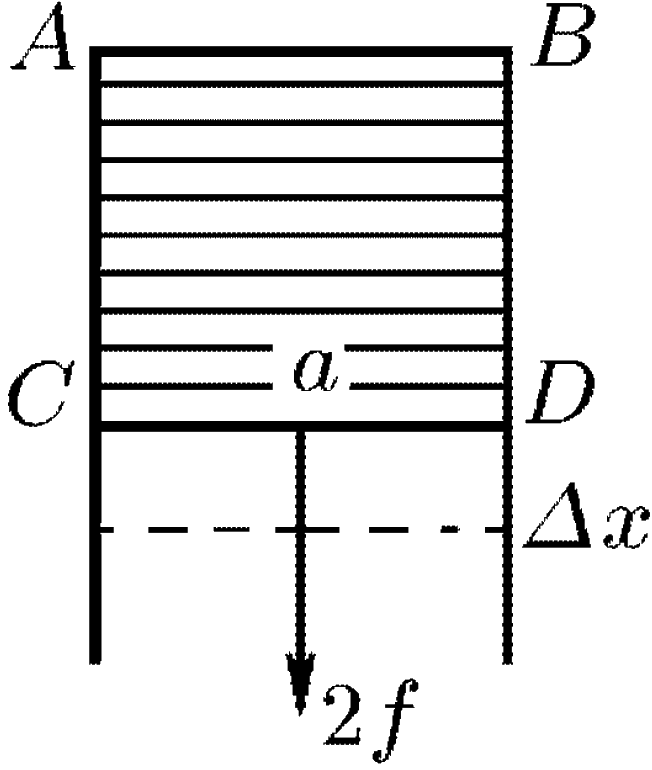
\includegraphics[width=30mm]{ris23_1.png}
\end{wrapfigure}
$$\sigma\equiv\dfrac{A}{\text{П}}\textbf{ --- коэффициент поверхностного натяжение, }$$
где $\text{П}\text{ --- площадь поверхности жидкости.}$ В изотермическом процессе работа идет на изменение $\Psi=\Psi_\text{об.}+\Psi_\text{пов.}$, где $\Psi_\text{об.}$ --- объемная энергия. $\Psi_\text{об.}\sim U$, а поверхностная энергия $\Psi_\text{пов.} =\sigma\text{П}$.
Пленка состоит из двух простых, значит $\delta A=2fdx$.
$$\sigma = \left(\dfrac{\delta A}{d\text{П}}\right)_T=\dfrac{2fdx}{2adx}=\dfrac{f}{a}$$
\begin{minipage}{55mm}
	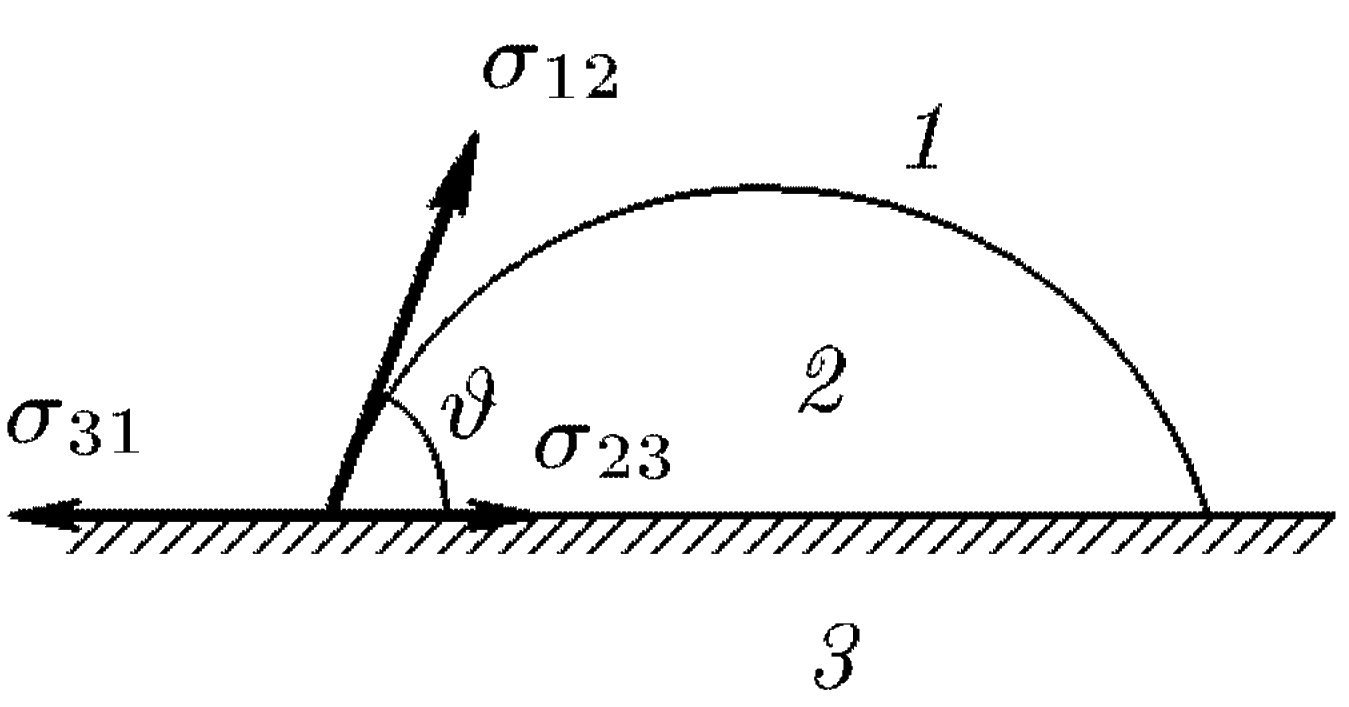
\includegraphics[width=50mm]{ris23_2.png}\\[-1cm] \center{a)}
\end{minipage}
\begin{minipage}{40mm}
	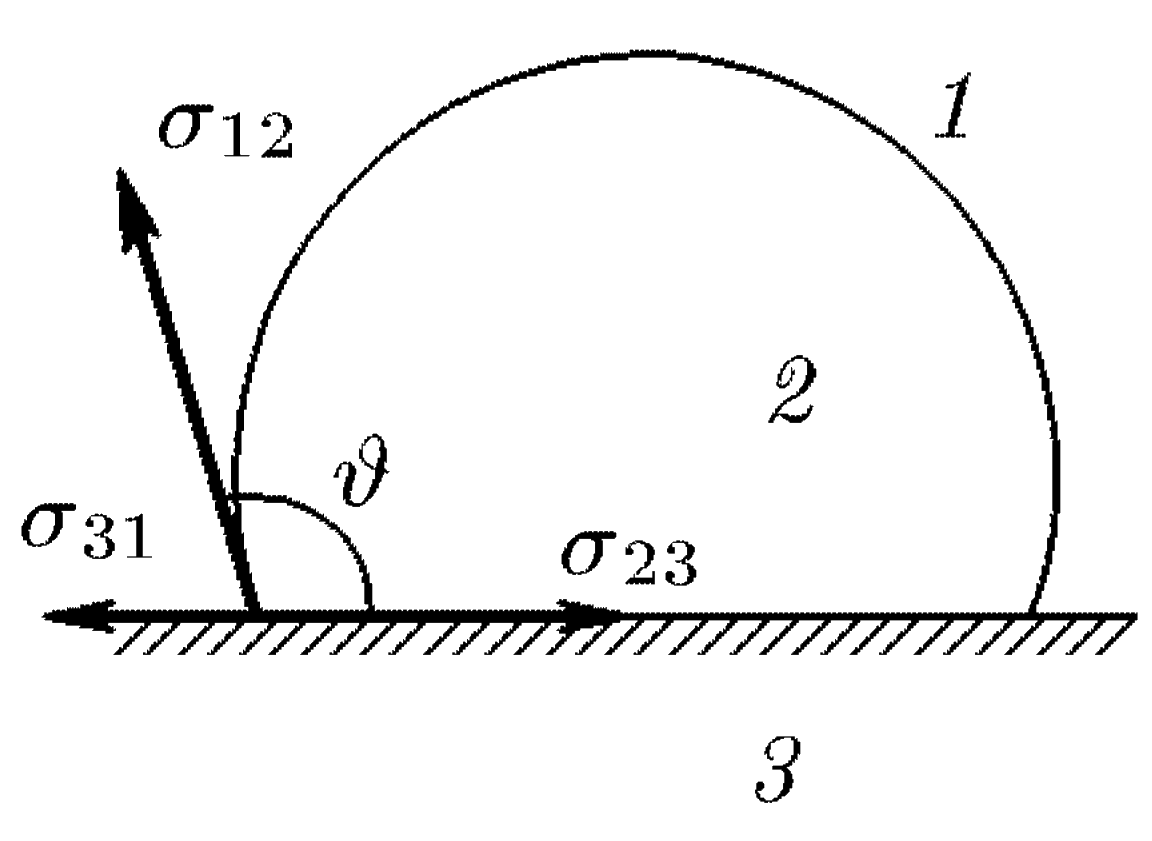
\includegraphics[width=35mm]{ris23_3.png} \\[-1cm] \center{б)}
\end{minipage}
\begin{minipage}{80mm}
	Равновесие: $\sigma_{31}+\sigma_{23}+\sigma_{12}cos\vartheta=0$, \\$\vartheta$ --- \textbf{краевой угол}..\\
	$\dfrac{\sigma_{13}-\sigma_{23}}{\sigma_{12}}>1$ --- \textbf{полное смачивание};\\
	$\dfrac{\sigma_{13}-\sigma_{23}}{\sigma_{12}}<-1$ --- \textbf{полное не смачивание};
\end{minipage}
Также если $0<\vartheta<\pi/2$, то имеет место \textbf{частичное смачивание}, а при $\pi/2<\vartheta<\pi$ --- \textbf{частичное не смачивание}.\\[0.5cm]
\begin{minipage}{55mm}
	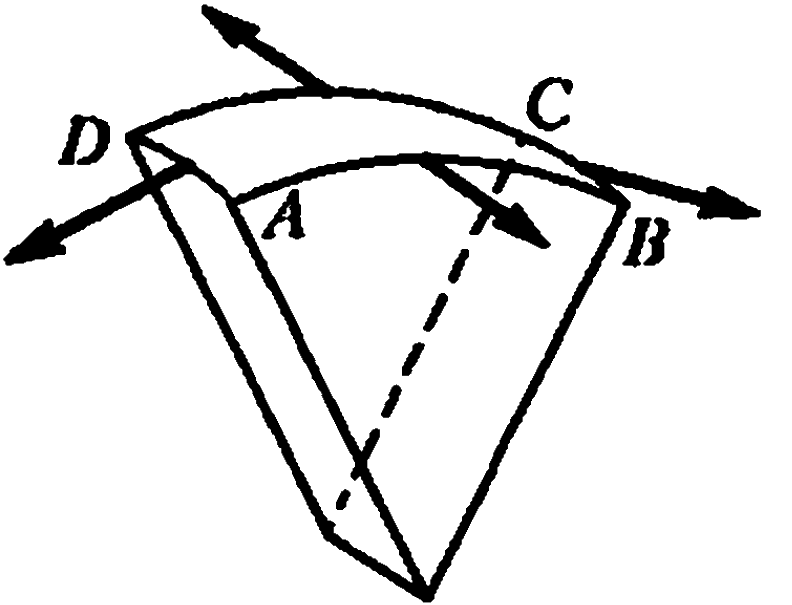
\includegraphics[width=50mm]{ris23_4.png}
	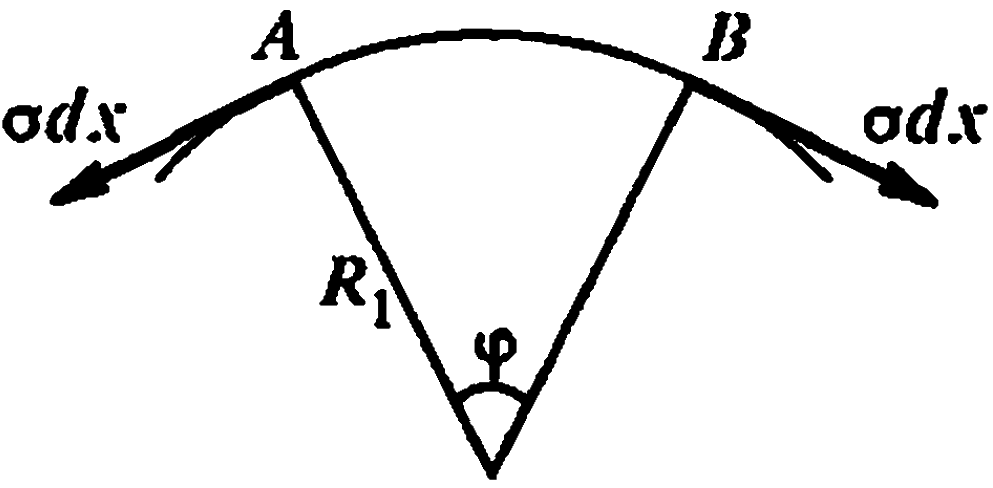
\includegraphics[width=50mm]{ris23_5.png}
\end{minipage}
\begin{minipage}{115mm}
	\paragraph{Формула Лапласа.}
	AD=$dx$, AB=$dy$ --- стороны прямоугольника, выделенного на кривой поверхности. Равнодействующая сил, приложенных к AD и BC направленна по радиусу и равна \\
	$dF_1=2\sigma dx\sin \varphi/2\simeq\sigma\varphi dx$, $\varphi=\dfrac{\text{AB}}{R_1}=\dfrac{dy}{R_1}\Rightarrow\\
	\Rightarrow dF_1=\dfrac{\sigma}{R_1}dxdy=\dfrac{\sigma}{R_1}d\text{П};
	\quad dF_2=\dfrac{\sigma}{R_2}d\text{П};\quad
	\\dF=dF_1+dF_2=\sigma\left(R_1^{-1}+R_2^{-1}\right)d\text{П}\Rightarrow$ $$P_2-P_1=\sigma\left(R_1^{-1}+R_2^{-1}\right)\textbf{ --- формула Лапласа}$$
	Для сферической поверхности: $\Delta p=\dfrac{2\sigma}{R}$, а для мыльного пузыря --- $\Delta P = (2\sigma)\dfrac{2}{R}=\dfrac{4\sigma}{R}$
\end{minipage}
\paragraph{Свободная энергия и внутренняя энергия поверхности.} По первому началу термодинамики: $\delta Q=dU+\delta A =dU-\sigma d\text{П}\Leftrightarrow dU=TdS+\sigma d\text{П}$\\
$\Psi=U-TS\Rightarrow d\Psi=-SdT+\sigma d\text{П}\Rightarrow S=-\chpr{\Psi}{T}{\text{П}}\Rightarrow\Psi=U+T\chpr{\Psi}{T}{\text{П}}$
$$U=\left(\sigma-T\dfrac{d\sigma}{dT}\right)\text{П --- внутренняя энергия поверхности}$$
Если расширение изотермическое, то надо сообщить $Q=\Delta U-\sigma\text{П}=-T\dfrac{d\sigma}{dT}d\text{П}\Rightarrow \\\Rightarrow q=-T\dfrac{d\sigma}{dT}$ --- теплота образования единицы поверхности пленки.
